% ATTENZIONE: Nei file secondari NON devi inserire \begin{document} o \end{document}.
\newpage

\chapterimage{Pictures/Indice.png}
\chapter{Convolutional Neural Networks and Computer Vision}\label{ch:convnets}

\section{Image Representation and the Imaging Process}

In computer vision, the fundamental objective is to interpret and reason about visual inputs. Digital images are typically formed via an optical camera model (such as the pinhole camera model) and subsequently digitized, as shown in Figure~\ref{fig:pinhole}.

\begin{figure}[htbp]
    \centering
    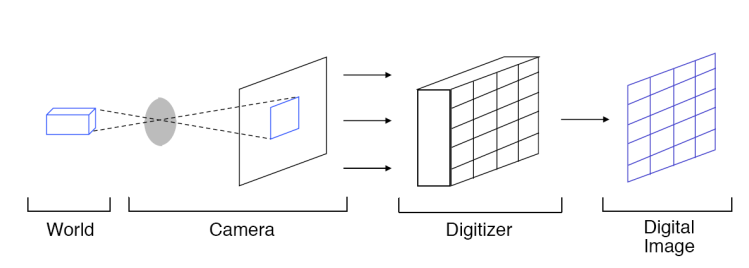
\includegraphics[width=0.7\textwidth]{Pictures/pinhole.png}
    \caption{Illustration of the pinhole camera imaging process.}\label{fig:pinhole}
\end{figure}

\begin{Notebox}
\textbf{The Digital Image Tensor:} A digital camera digitizes incoming light into a 3D array of numbers with dimensions $(H \times W \times C)$, where $H$ is the image height, $W$ is the image width, and $C$ represents the color channels (typically $C=3$ for Red, Green, and Blue). Each pixel intensity is represented by an integer in $[0, 255]$ or normalized as a floating-point value in $[0, 1]$.
\end{Notebox}

---

\section{Motivations for Convolutions}

\subsection{The Problem with Fully Connected Layers}

In standard Fully Connected (Dense) layers, every input unit is wired to every output unit. When applied directly to image data, this architecture exhibits severe failure modes:

\begin{itemize}[leftmargin=*]
    \item \textbf{Parameter Explosion \& Overfitting:} Consider a modest $1000 \times 1000$ RGB image ($3 \times 10^6$ input values). Connecting this input to a hidden layer of only $10^3$ neurons requires over $3 \times 10^9$ parameters (3 billion weights). Storing and optimizing this volume of parameters requires unfeasible memory and inevitably triggers catastrophic overfitting.
    \item \textbf{Destruction of Spatial Topology:} Flattening an image into a 1D vector completely ignores spatial relationships, treating adjacent pixels with the same prior relevance as pixels located at opposite ends of the image.
\end{itemize}

\subsection{Exploiting Image Structure: Locality and Stationarity}

To overcome these structural limitations, \textbf{Convolutional Neural Networks (CNNs)} leverage two intrinsic physical properties of visual data:

\begin{enumerate}
    \item \textbf{Local Spatial Correlation:} Spatially proximal pixels exhibit strong statistical correlation, whereas distant pixels are relatively uncorrelated. Instead of connecting each neuron globally to the entire image, a neuron connects only to a small local receptive field.
    \item \textbf{Translation Stationarity (Invariance):} Visual features (such as edges, corners, and textures) are statistically invariant to spatial translation. A pattern detector useful in the top-left corner is equally meaningful in the bottom-right corner. Consequently, the same set of parameters can be shared across all spatial positions.
\end{enumerate}

---

\section{The Core Building Block: The Convolutional Layer}

\begin{figure}[htbp]
    \centering
    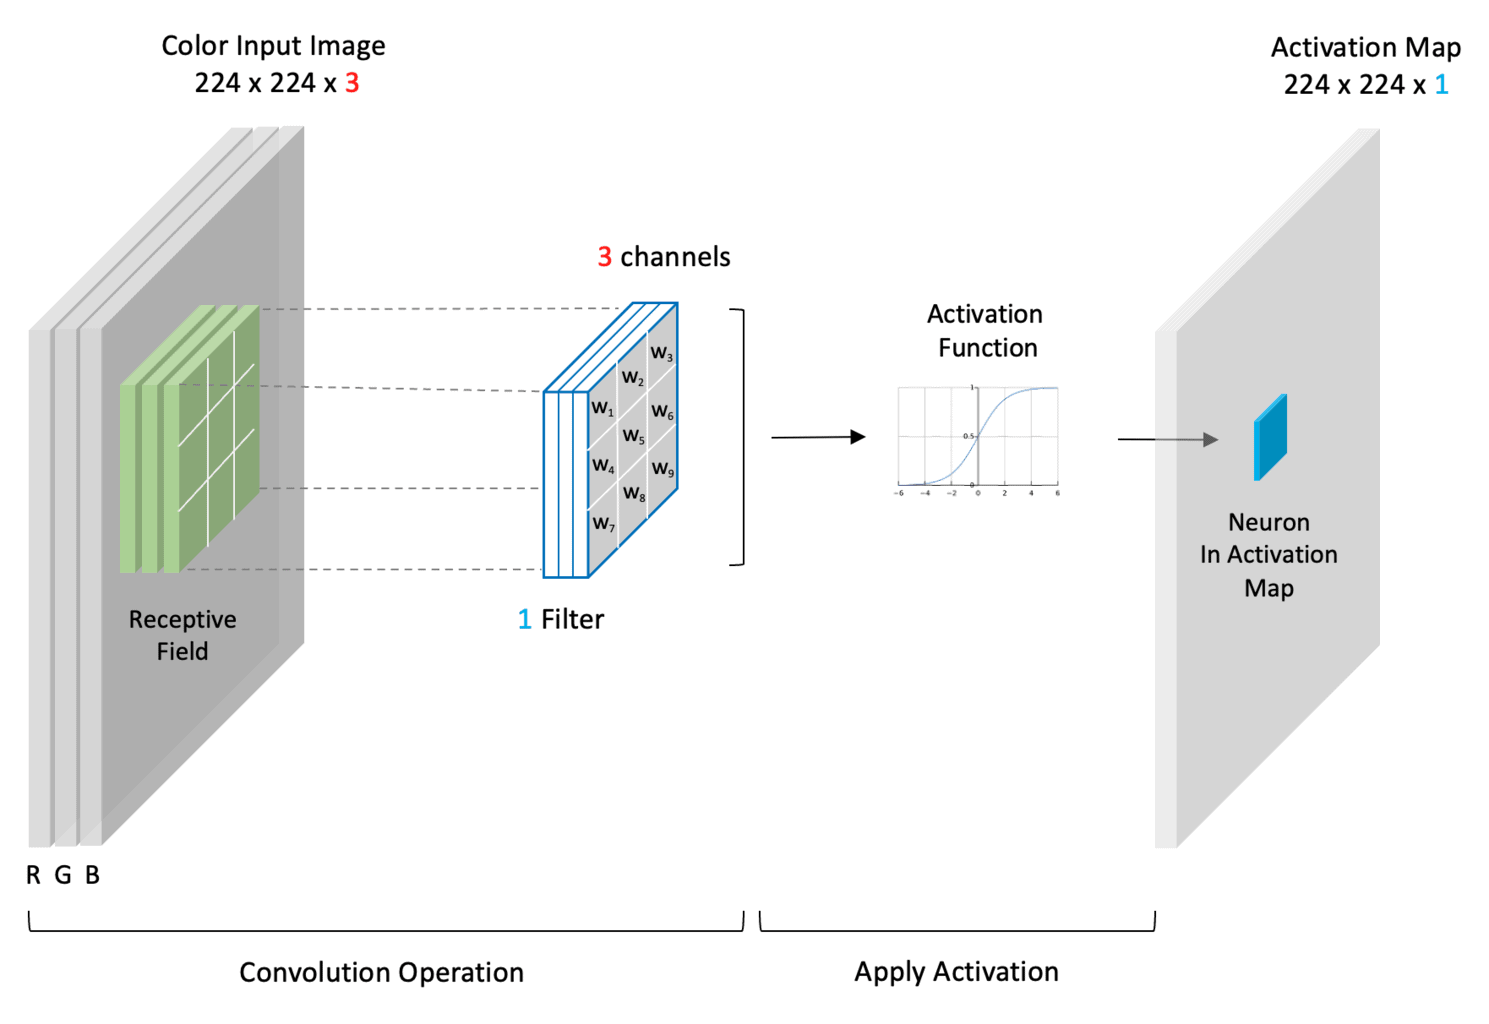
\includegraphics[width=0.7\textwidth]{Pictures/convolutional_layer_example.png}
    \caption{Illustration of a single convolutional layer operating on an image.}\label{fig:convolutional_layer_example}
\end{figure}

A Convolutional Layer replaces dense matrix multiplication with a local sliding operation, illustrated in Figure~\ref{fig:convolutional_layer_example}:

\begin{itemize}[leftmargin=*]
    \item \textbf{The Kernel (Filter):} A small matrix of learnable weights (e.g., $3 \times 3$ or $5 \times 5$). It serves as a specialized feature detector.
    \item \textbf{The Sliding Window:} The filter slides systematically across the spatial grid of the input. At each position, it computes the dot product (sum of element-wise multiplications) between its weights and the underlying local patch.
    \item \textbf{The Feature Map:} The resulting output grid, illustrated in Figure~\ref{fig:featuremap}. High values indicate strong alignment between the learned filter pattern and that specific image region.
\end{itemize}

\begin{figure}[htbp]
    \centering
    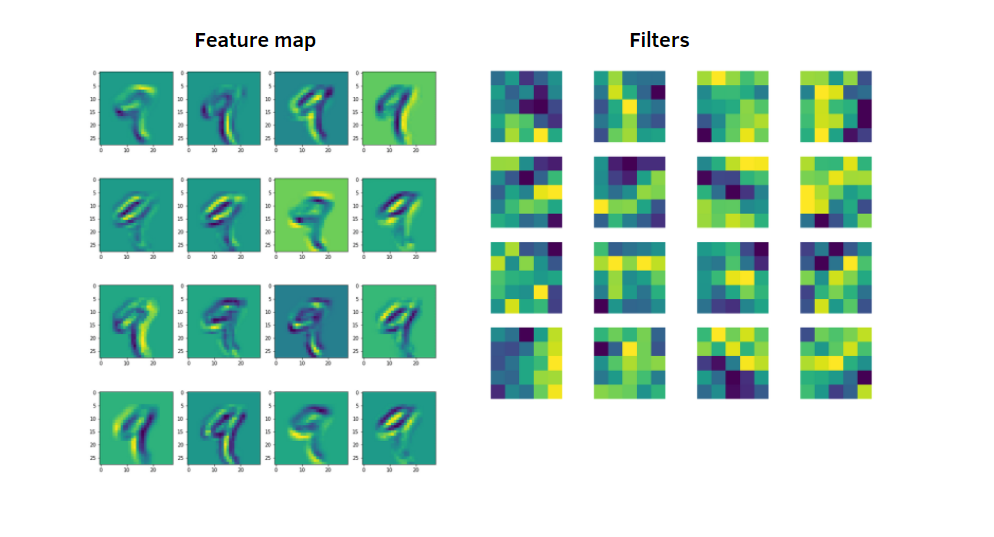
\includegraphics[width=0.7\textwidth]{Pictures/conv_feature_map.png}
    \caption{Multiple feature maps produced by convolving distinct filters over an input.}\label{fig:featuremap}
\end{figure}

\subsection{Key Hyperparameters of the Convolution}

The behavior and spatial dimensions of a convolutional layer are governed by three primary hyperparameters:

\begin{itemize}[leftmargin=*]
    \item \textbf{Stride ($S$):} The step size with which the kernel moves across the image. A stride of $S=1$ moves pixel-by-pixel, while $S > 1$ downsamples the output grid.
    \item \textbf{Padding ($P$):} Adding zero-valued borders around the input image boundary to preserve spatial dimensions and ensure edge pixels receive equal computational attention.
    \item \textbf{Channels ($C$):} Real images have depth (e.g., $C_{in} = 3$ for RGB). A kernel must match the depth of the input, yielding a 3D tensor of shape $(C_{in} \times K_h \times K_w)$. Using $C_{out}$ distinct kernels produces $C_{out}$ output feature maps.
\end{itemize}

\subsection{Formal Mathematical Definition}

Formally, the discrete 2D convolution of an image $I$ with a 2D filter $g$ at spatial location $[m, n]$ is defined as:

\begin{equation}
f[m, n] = (I * g)[m, n] = \sum_{k} \sum_{l} I[m - k, n - l] \, g[k, l]
\label{eq:2d_conv}
\end{equation}
where $k$ and $l$ index the spatial extent of the kernel.

\begin{keywordbox}
\textbf{Convolution versus Cross-Correlation in Deep Learning} \\
In classical signal processing, the index subtraction $I[m - k, n - l]$ implies flipping the kernel $g$ by $180^\circ$. 
Deep learning libraries (e.g., PyTorch) compute \textbf{Cross-Correlation} instead:
\[ f[m, n] = (I \star g)[m, n] = \sum_{k} \sum_{l} I[m + k, n + l] \, g[k, l] \]
Because kernel weights $g[k, l]$ are learned from scratch via backpropagation, the network simply learns pre-flipped weights directly, rendering cross-correlation and convolution mathematically equivalent for optimization.
\end{keywordbox}

---

\section{Classic Image Processing Filters}

Before inspecting multi-channel deep representations, consider how classical handcrafted kernels manipulate local spatial neighborhoods to extract specific visual features.

\begin{examplebox}
\textbf{1. Smoothing Filter (Noise Reduction):}\\
Replacing each pixel with a weighted neighborhood average dampens noise and sharp outliers:
\[
\begin{array}{|c|c|c|}
\hline
2 & 3 & 3 \\ \hline
3 & \mathbf{20} & 2 \\ \hline
3 & 2 & 3 \\ \hline
\end{array}
\quad \xrightarrow{\text{Smoothing}} \quad
\begin{array}{|c|c|c|}
\hline
2 & 3 & 3 \\ \hline
3 & \mathbf{3} & 2 \\ \hline
3 & 2 & 3 \\ \hline
\end{array}
\]
The central anomaly ($20$) is effectively smoothed down to $3$.
\end{examplebox}

\begin{examplebox}
\textbf{2. Vertical Edge Detection Filter:}\\
Filters with opposing positive and negative signs detect sharp directional variations in pixel intensity:
\[
g_{\text{vertical}} = \begin{array}{|c|c|c|}
\hline
-1 & 0 & 1 \\ \hline
-1 & 0 & 1 \\ \hline
-1 & 0 & 1 \\ \hline
\end{array}
\]
Transposing $g_{\text{vertical}}$ yields a horizontal edge detector $g_{\text{horizontal}} = g_{\text{vertical}}^T$.
\end{examplebox}

\begin{examplebox}
\textbf{3. Step-by-Step 2D Convolution Example (Stride 1, Pad 1):}\\
Convolving a $3 \times 3$ image $I$ with a vertical edge filter $g$ with padding $P = 1$ pads the input with zeros into a $5 \times 5$ grid $I_{\text{padded}}$:
\[
I_{\text{padded}} = 
\begin{array}{|c|c|c|c|c|}
\hline
0 & 0 & 0 & 0 & 0 \\ \hline
0 & 8 & 5 & 2 & 0 \\ \hline
0 & 7 & 5 & 3 & 0 \\ \hline
0 & 9 & 4 & 1 & 0 \\ \hline
0 & 0 & 0 & 0 & 0 \\ \hline
\end{array}
\]
Applying the convolution with stride $S = 1$ yields:
\[
\begin{array}{c} g[k,l] \\ \begin{array}{|c|c|c|}
\hline
-1 & 0 & 1 \\ \hline
-1 & 0 & 1 \\ \hline
-1 & 0 & 1 \\ \hline
\end{array} \end{array}
\quad \otimes \quad
\begin{array}{c} I_{\text{padded}} \\ \text{\small(conceptually)} \end{array}
\quad = \quad
\begin{array}{c} f[m,n] \\ \begin{array}{|c|c|c|}
\hline
-10 & 10 & 10 \\ \hline
-14 & 18 & 14 \\ \hline
-9 & 12 & 9 \\ \hline
\end{array} \end{array}
\]

\textbf{Accounting for the $180^\circ$ Kernel Flip:}\\
Flipping $g$ by $180^\circ$ produces:
\[
g_{\text{flipped}} = \begin{array}{|c|c|c|}
\hline
1 & 0 & -1 \\ \hline
1 & 0 & -1 \\ \hline
1 & 0 & -1 \\ \hline
\end{array}
\]
\begin{itemize}[nosep, leftmargin=*]
    \item \textbf{Center Value $f[1,1] = 18$:} Flipped kernel overlaps fully with the original $3 \times 3$ image pixels:
    \[ (1 \cdot 8 - 1 \cdot 2) + (1 \cdot 7 - 1 \cdot 3) + (1 \cdot 9 - 1 \cdot 1) = 6 + 4 + 8 = 18 \]
    \item \textbf{Top-Left Value $f[0,0] = -10$:} Flipped kernel overlaps with the top-left boundary of $I_{\text{padded}}$:
    \[ (1 \cdot 0 - 1 \cdot 5) + (1 \cdot 0 - 1 \cdot 5) = -10 \]
\end{itemize}
\end{examplebox}

---

\section{Output Shape and Parameter Counting for 3D Volumes}

In deep vision models, inputs are 3D tensors $(C_{\text{in}} \times H \times W)$, and each layer applies a bank of $C_{\text{out}}$ distinct filters.

\subsection{Spatial Output Size Formula}
Given an input spatial width $W$, kernel spatial size $K$, padding $P$, and stride $S$, the output spatial width $W_{\text{out}}$ is given by:

\begin{equation}
W_{\text{out}} = \left\lfloor \frac{W - K + 2P}{S} \right\rfloor + 1
\label{eq:spatial_output_size}
\end{equation}

\begin{examplebox}
\textbf{Numerical Example of Parameter Counting:}\\
Suppose the input volume is a $32 \times 32 \times 3$ image, and we apply $10$ filters of size $5 \times 5$ (with stride $S = 1$, padding $P = 2$):
\begin{itemize}[nosep, leftmargin=*]
    \item \textbf{Output spatial size:} $\lfloor(32 - 5 + 2 \cdot 2)/1\rfloor + 1 = 32 \implies (32 \times 32)$.
    \item \textbf{Output volume size:} $32 \times 32 \times 10$.
    \item \textbf{Number of parameters:} Each filter has $5 \times 5 \times 3 = 75$ weights plus $1$ bias $= 76$ parameters. For 10 filters: $76 \times 10 = \mathbf{760\text{ parameters}}$.
\end{itemize}
\end{examplebox}

---

\section{The Pooling Layer}

Convolutional neural networks interleave convolutional layers with \textbf{Pooling layers} to perform spatial downsampling.

\subsection{Purpose and Properties of Pooling}
\begin{itemize}[nosep, leftmargin=*]
    \item \textbf{Spatial Dimensionality Reduction:} Reduces spatial width and height, reducing computational complexity in deeper layers.
    \item \textbf{Parameter Control:} Shrinking feature map resolutions minimizes the number of parameters needed when eventually transitioning to fully connected classification heads.
    \item \textbf{Translation Invariance:} Pooling provides slight invariance to local translations; small shifts in the input do not alter the pooled maximum or mean.
    \item \textbf{Channel Independence:} Pooling operates independently on each depth slice without mixing channels. If the input has $C$ channels, the output has exactly $C$ channels.
\end{itemize}

\subsection{Max Pooling}
Max Pooling slides a window across each channel and outputs strictly the \textbf{maximum value} in each receptive window.

\begin{examplebox}
\textbf{Max Pooling Example ($2 \times 2$ filter, Stride 2):}\\
Applying Max Pooling to a $4 \times 4$ slice:
\[
\begin{array}{|c|c|c|c|}
\hline
1 & 1 & 2 & 4 \\ \hline
5 & 6 & 7 & 8 \\ \hline
3 & 2 & 1 & 0 \\ \hline
1 & 2 & 3 & 4 \\ \hline
\end{array}
\quad \xrightarrow{\text{Max Pool } 2 \times 2, S=2} \quad
\begin{array}{|c|c|}
\hline
6 & 8 \\ \hline
3 & 4 \\ \hline
\end{array}
\]
Spatial dimensions are halved, discarding $75\%$ of activations and retaining only the most prominent local features.
\end{examplebox}

\subsection{Average Pooling}
Average Pooling computes the \textbf{arithmetic mean} over each local window:

\begin{examplebox}
\textbf{Average Pooling Example ($2 \times 2$ filter, Stride 2):}\\
Applying Average Pooling to a $4 \times 4$ slice:
\[
\begin{array}{|c|c|c|c|}
\hline
1 & 1 & 2 & 4 \\ \hline
4 & 6 & 6 & 8 \\ \hline
3 & 2 & 1 & 0 \\ \hline
1 & 2 & 3 & 4 \\ \hline
\end{array}
\quad \xrightarrow{\text{Average Pool } 2 \times 2, S=2} \quad
\begin{array}{|c|c|}
\hline
3 & 5 \\ \hline
2 & 2 \\ \hline
\end{array}
\]
\end{examplebox}

---

\section{Visualizing Convolutional Networks}

\begin{InsightBox}
Visualizing what deep CNNs learn (e.g., via Deconvolutional Networks by Zeiler and Fergus) reveals a clear hierarchical decomposition:
\begin{itemize}[nosep, leftmargin=*]
    \item \textbf{Layer 1:} Learns elementary low-level visual primitives (oriented edges, basic color gradients).
    \item \textbf{Layer 2:} Combines primitives into textures, corners, and simple geometric patterns.
    \item \textbf{Layer 3 and Deeper:} Assembles textures into semantically complex object parts (e.g., wheels, faces) and eventually full objects.
\end{itemize}
\end{InsightBox}

\begin{figure}[htbp]
    \centering
    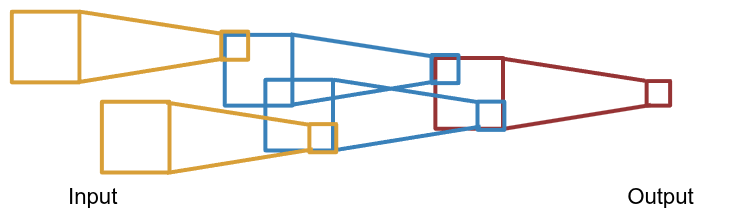
\includegraphics[width=0.5\textwidth]{Pictures/in_out.png}
    \caption{Hierarchical feature representations learned across deep convolutional layers.}\label{fig:inout}
\end{figure}

---

\section{Vision Regularization: Data Augmentation}

While weight decay acts on model parameters and Dropout acts on activations, \textbf{Data Augmentation} acts directly on the input data. It artificially expands training dataset diversity by applying label-preserving transformations, embodying the standard modern regularization paradigm: introducing stochasticity at training and evaluating on fixed standard inputs at test time.

\subsection{Classic Spatial and Color Augmentations}
\begin{itemize}[leftmargin=*]
    \item \textbf{Horizontal Flips:} A simple, highly effective transformation for general object recognition.
    \item \textbf{Random Crops and Scales:} During training, random patches are extracted at varying scales (e.g., ResNet resizes the short side between 256 and 480 pixels before extracting a $224 \times 224$ crop). At test time, predictions are averaged over a fixed set of crops (e.g., 10 crops: 4 corners + center, and their horizontal flips).
    \item \textbf{Color Jitter:} Perturbing brightness, contrast, and saturation to render the model invariant to illumination changes.
\end{itemize}

\begin{figure}[htbp]
    \centering
    \begin{minipage}{0.48\textwidth}
        \centering
        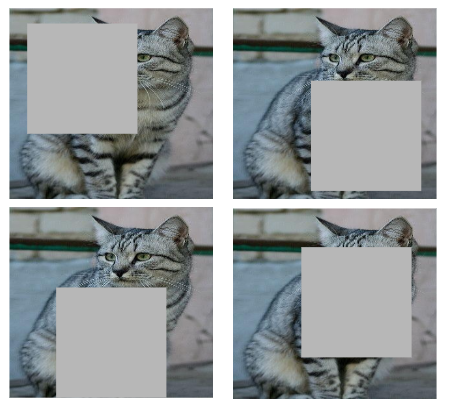
\includegraphics[width=\linewidth]{Pictures/catcutout.png}
        \caption{Example of Cutout.}\label{fig:cutout}
    \end{minipage}\hfill
    \begin{minipage}{0.48\textwidth}
        \centering
        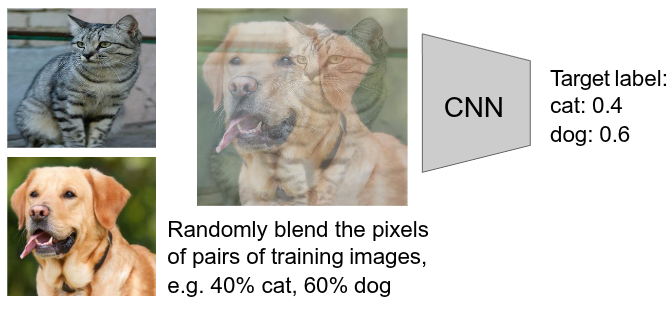
\includegraphics[width=\linewidth]{Pictures/mixup.png}
        \caption{Example of Mixup.}\label{fig:mixup}
    \end{minipage}
\end{figure}

\subsection{Advanced Stochastic Augmentations}
\begin{itemize}[leftmargin=*]
    \item \textbf{Cutout:} During training, square image patches are randomly masked out (set to zero). This forces the network to avoid over-relying on a single dominant feature (such as an animal's face) and learn distributed contextual cues. Unmodified images are evaluated at test time.
    \item \textbf{Mixup (Zhang et al., 2018):} Blends pairs of images and their corresponding one-hot labels linearly. For instance, blending $40\%$ of a cat image with $60\%$ of a dog image produces a target training label of $[0.4\,\text{cat}, 0.6\,\text{dog}]$. At test time, standard unblended images are used.
\end{itemize}

---

\section{Transfer Learning in Computer Vision}

\subsection{The Fundamental Concept (Why Use It?)}
Training deep Convolutional Neural Networks from scratch requires massive datasets (e.g., millions of annotated images). On small target datasets, training from scratch leads to severe overfitting.

The solution is \textbf{Transfer Learning}: leveraging a \textbf{Source model} pre-trained on a gigantic dataset (e.g., ImageNet) and transferring its learned visual representations to a \textbf{Target model} for a specific, smaller task.

\subsection{Practical Implementation}
Using standard backbones like VGG or ResNet, transfer learning proceeds in two stages:
\begin{itemize}[leftmargin=*]
    \item \textbf{1. Preserving Convolutional Feature Extractors:} Early and middle convolutional layers are kept frozen. They act as universal feature extractors, having already learned edge, texture, and shape primitives common to all natural visual scenes.
    \item \textbf{2. Replacing the Classification Head:} The final Fully Connected layers are removed and replaced with new layers configured for the target dataset's classes. Only this new head (and optionally fine-tuned upper conv layers) is trained.
\end{itemize}

\subsection{Pervasiveness: The Modern Standard}
Transfer learning is standard across all computer vision applications:
\begin{itemize}[leftmargin=*]
    \item \textbf{Object Detection:} Frameworks like Fast R-CNN utilize ImageNet-pre-trained CNN backbones to extract spatial features before predicting bounding boxes.
    \item \textbf{Image Captioning:} Pre-trained CNN backbones produce dense feature vectors that initialize or condition recurrent sequence decoders.
\end{itemize}

\begin{keywordbox}
\textbf{The Model Zoo} \\
All major deep learning frameworks provide a **Model Zoo** (e.g., \texttt{torchvision.models} in PyTorch) containing pre-trained weights for state-of-the-art vision architectures. These models can be downloaded instantly and fine-tuned for custom downstream tasks.
\end{keywordbox}

\newpage
\section{Chapter Summary and Conceptual Graph}

The concepts developed in this chapter establish how the inductive biases of natural visual data lead from raw pixels to deep hierarchical vision systems:

\begin{InsightBox}
\textbf{The Logical Connections Between Nodes:}
\begin{itemize}[leftmargin=*]
    \item \textbf{From Node 1 to 2:} Viewing digital images as raw flattened arrays reveals why generic architectures fail: high spatial resolutions lead directly to parameter explosion and loss of geometry.
    \item \textbf{From Node 2 to 3:} Recognizing the failure of dense connections motivates identifying domain-specific inductive biases: pixels exhibit local correlation and patterns are invariant to spatial shifts.
    \item \textbf{From Node 3 to 4:} Locality and stationarity directly dictate the mathematical structure of the Convolutional Layer: local receptive fields with shared kernel weights.
    \item \textbf{From Node 4 to 5:} While convolutions preserve spatial structure, deep networks need downsampling to grow the effective receptive field and limit computation, achieved through parameter-free Pooling layers.
    \item \textbf{From Node 5 to 6:} Interleaving convolutions and pooling enables deep networks to naturally learn hierarchical representations, moving from oriented edges in early layers to semantic concepts in deep layers.
    \item \textbf{From Node 6 to 7:} Deep vision models with high expressive capacity easily memorize training images; Data Augmentation (including Cutout and Mixup) enforces invariance to photometric and spatial perturbations.
    \item \textbf{From Node 7 to 8:} Because training deep CNNs from scratch requires millions of images, Transfer Learning allows small custom datasets to inherit universal visual features from large-scale pre-trained Model Zoos.
\end{itemize}
\end{InsightBox}

\begin{figure}[htbp]
\centering
\begin{tikzpicture}[
    node distance=0.6cm and 0cm,
    conceptnode/.style={
        rectangle, rounded corners=4pt, draw=ocre!80, fill=ocre!8,
        line width=0.8pt, text width=0.85\textwidth, inner sep=5pt,
        font=\sffamily\small
    },
    arrowline/.style={
        ->, >=Stealth, line width=1pt, color=ocre!80
    }
]

\node[conceptnode] (n1) {\textbf{1. Digital Image Representation}\\
Continuous optical images digitized into multi-dimensional pixel arrays $(H \times W \times C)$.};

\node[conceptnode, below=of n1] (n2) {\textbf{2. Failure of Fully Connected Layers}\\
Dense connections explode parameter counts into billions and ignore 2D spatial grid topology.};

\node[conceptnode, below=of n2] (n3) {\textbf{3. Inductive Biases: Locality \& Stationarity}\\
Physical priors of images: nearby pixels correlate (local receptive fields); features are translation-invariant (weight sharing).};

\node[conceptnode, below=of n3] (n4) {\textbf{4. The Convolutional Layer}\\
Learnable 2D/3D kernels slide across the spatial grid, computing local cross-correlations to produce feature maps.};

\node[conceptnode, below=of n4] (n5) {\textbf{5. Pooling Layers (Max \& Average)}\\
Subsamples spatial dimensions to reduce computation and induce local translation invariance without parameters.};

\node[conceptnode, below=of n5] (n6) {\textbf{6. Hierarchical Visual Representations}\\
Deep stacking naturally discovers compositional primitives: low-level edges $\to$ textures $\to$ object parts $\to$ semantic classes.};

\node[conceptnode, below=of n6] (n7) {\textbf{7. Vision Regularization: Data Augmentation}\\
Artificially expands dataset diversity via spatial crops, flips, Cutout, and Mixup to prevent overfitting.};

\node[conceptnode, below=of n7] (n8) {\textbf{8. Transfer Learning \& Model Zoos}\\
Overcomes small-data limitations by freezing pre-trained CNN backbones and adapting only classification heads.};

\draw[arrowline] (n1) -- (n2);
\draw[arrowline] (n2) -- (n3);
\draw[arrowline] (n3) -- (n4);
\draw[arrowline] (n4) -- (n5);
\draw[arrowline] (n5) -- (n6);
\draw[arrowline] (n6) -- (n7);
\draw[arrowline] (n7) -- (n8);

\end{tikzpicture}
\caption{Conceptual roadmap of convolutional neural networks and computer vision.}\label{fig:ch2_roadmap}
\end{figure}
